\documentclass[border=10pt]{standalone}
\usepackage{amsmath}
\usepackage{amssymb}
\usepackage{tikz}
\usetikzlibrary{arrows.meta,calc,decorations.pathreplacing,patterns,shapes.geometric,positioning,shadings,plotmarks}

\begin{document}
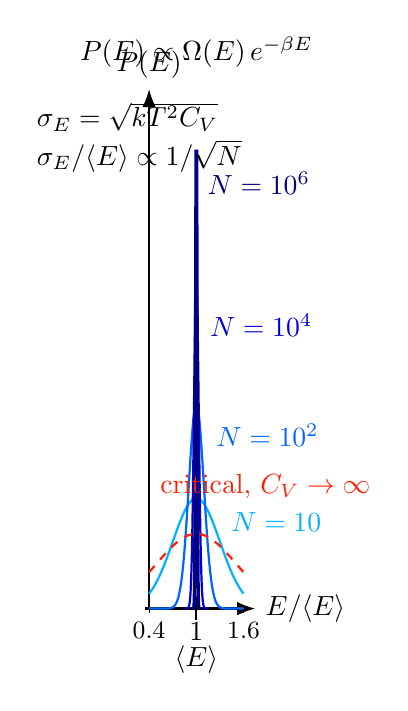
\begin{tikzpicture}[>=Latex]

% Axes
\def\xmin{0.4}
\def\xmax{1.6}
\def\ymax{6.2}
\draw[->, thick] (\xmin-0.05,0) -- (\xmax+0.15,0) node[right] {$E/\langle E\rangle$};
\draw[->, thick] (\xmin,0) -- (\xmin,\ymax+0.4) node[above] {$P(E)$};

% Title
\node[anchor=south] at (1.0,\ymax+0.55) {$P(E)\propto \Omega(E)\,e^{-\beta E}$};

% X-axis ticks
\draw (1.0,0.05) -- (1.0,-0.05) node[below] {$1$};
\draw (\xmin,0.05) -- (\xmin,-0.05) node[below] {\small $0.4$};
\draw (\xmax,0.05) -- (\xmax,-0.05) node[below] {\small $1.6$};

% Mark <E> position with short vertical line
\draw[thick] (1.0,-0.15) -- (1.0,0.15);
\node[anchor=north] at (1.0,-0.35) {$\langle E\rangle$};

% Gaussian curves with widths sigma proportional to 1/sqrt(N)
% sigma values chosen so adjacent ratio ~ sqrt(10) ~ 3.16
% Heights normalized: peak = A/sigma so area constant; we'll scale to fit

% N=10:    sigma = 0.30   peak ~ 1.33/0.30 = 4.43  -> use peak 1.4
% N=10^2:  sigma = 0.095  peak ~ 1.40/0.095 ~ 14.7  too tall -> scale
% Better: pick visible peaks manually with widths in correct ratio

% Light blue (N=10), width sigma1 = 0.30, peak h1 = 1.4
\draw[color=blue!30!cyan, thick, smooth, samples=200, domain=\xmin:\xmax]
  plot (\x, {1.4*exp(-((\x-1)*(\x-1))/(2*0.30*0.30))});

% Medium blue (N=10^2), sigma2 = 0.095, peak h2 = 2.6
\draw[color=blue!60!cyan, thick, smooth, samples=200, domain=\xmin:\xmax]
  plot (\x, {2.6*exp(-((\x-1)*(\x-1))/(2*0.095*0.095))});

% Darker blue (N=10^4), sigma3 = 0.030, peak h3 = 4.2
\draw[color=blue!85!black, thick, smooth, samples=300, domain=0.85:1.15]
  plot (\x, {4.2*exp(-((\x-1)*(\x-1))/(2*0.030*0.030))});

% Deep blue (N=10^6), sigma4 = 0.0095, peak h4 = 5.8
\draw[color=blue!50!black, very thick, smooth, samples=400, domain=0.95:1.05]
  plot (\x, {5.8*exp(-((\x-1)*(\x-1))/(2*0.0095*0.0095))});

% Critical anomalous curve (dashed warm red), wider than N=10 (use sigma_c = 0.50)
\draw[color=red!75!orange, thick, dashed, smooth, samples=200, domain=\xmin:\xmax]
  plot (\x, {0.95*exp(-((\x-1)*(\x-1))/(2*0.50*0.50))});

% Curve labels
\node[color=blue!30!cyan, anchor=west] at (1.32,1.1) {$N=10$};
\node[color=blue!60!cyan, anchor=west] at (1.13,2.2) {$N=10^2$};
\node[color=blue!85!black, anchor=west] at (1.05,3.6) {$N=10^4$};
\node[color=blue!50!black, anchor=west] at (1.02,5.4) {$N=10^6$};
\node[color=red!75!orange, anchor=west, align=left] at (0.42,1.55) {critical, $C_V\to\infty$};

% Right-side equation box
\node[anchor=north east, align=left] at (\xmax+0.1,\ymax+0.35)
  {$\sigma_E = \sqrt{kT^2 C_V}$ \\[2pt] $\sigma_E/\langle E\rangle \propto 1/\sqrt{N}$};

\end{tikzpicture}
\end{document}
